\documentclass{standalone}
\usepackage{tikz}
\usetikzlibrary{patterns, positioning}

\begin{document}
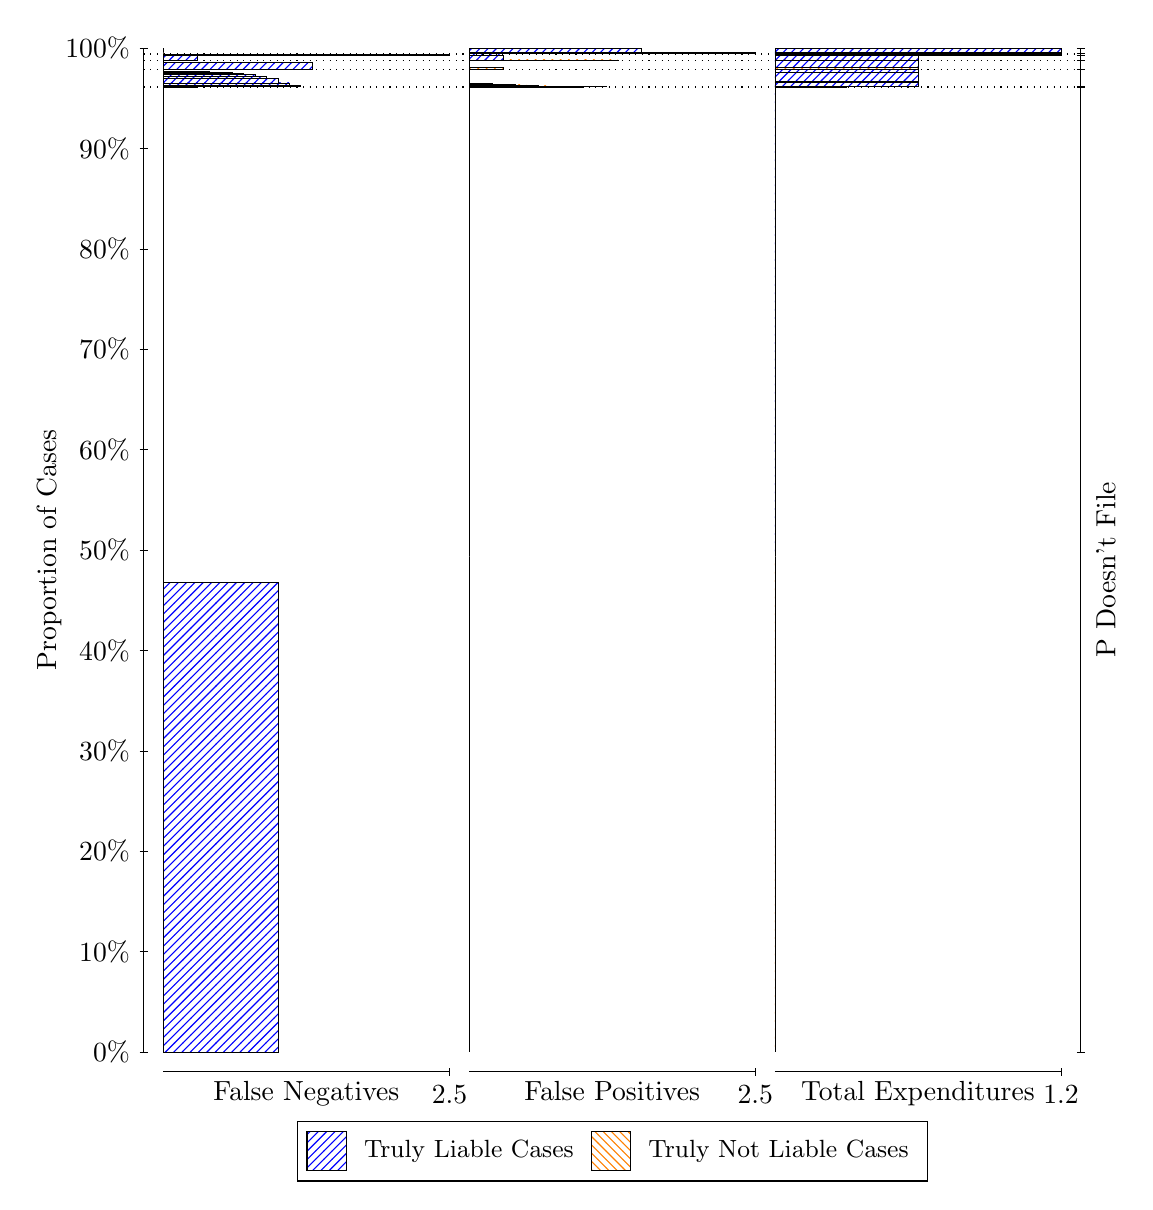
\begin{tikzpicture}
\draw[black, very thin] (1.5,1.75) -- (1.5,14.5);
\node[rotate=90, anchor=center] at (0.3, 8.125) {Proportion of Cases};
\draw[black, very thin] (1.45,1.75) -- (1.55,1.75);
\node[anchor=east] at (1.45, 1.75) {0\%};
\draw[black, very thin] (1.45,3.025) -- (1.55,3.025);
\node[anchor=east] at (1.45, 3.025) {10\%};
\draw[black, very thin] (1.45,4.3) -- (1.55,4.3);
\node[anchor=east] at (1.45, 4.3) {20\%};
\draw[black, very thin] (1.45,5.575) -- (1.55,5.575);
\node[anchor=east] at (1.45, 5.575) {30\%};
\draw[black, very thin] (1.45,6.85) -- (1.55,6.85);
\node[anchor=east] at (1.45, 6.85) {40\%};
\draw[black, very thin] (1.45,8.125) -- (1.55,8.125);
\node[anchor=east] at (1.45, 8.125) {50\%};
\draw[black, very thin] (1.45,9.4) -- (1.55,9.4);
\node[anchor=east] at (1.45, 9.4) {60\%};
\draw[black, very thin] (1.45,10.675) -- (1.55,10.675);
\node[anchor=east] at (1.45, 10.675) {70\%};
\draw[black, very thin] (1.45,11.95) -- (1.55,11.95);
\node[anchor=east] at (1.45, 11.95) {80\%};
\draw[black, very thin] (1.45,13.225) -- (1.55,13.225);
\node[anchor=east] at (1.45, 13.225) {90\%};
\draw[black, very thin] (1.45,14.5) -- (1.55,14.5);
\node[anchor=east] at (1.45, 14.5) {100\%};

\draw[black, very thin] (13.4,1.75) -- (13.4,14.5);
\draw[black, very thin] (13.35,1.75) -- (13.45,1.75);
\node[anchor=west] at (13.35, 1.75) {};
\draw[black, very thin] (13.35,13.999) -- (13.45,13.999);
\node[anchor=west] at (13.35, 13.999) {};
\draw[black, very thin] (13.35,14.008) -- (13.45,14.008);
\node[anchor=west] at (13.35, 14.008) {};
\draw[black, very thin] (13.35,14.231) -- (13.45,14.231);
\node[anchor=west] at (13.35, 14.231) {};
\draw[black, very thin] (13.35,14.341) -- (13.45,14.341);
\node[anchor=west] at (13.35, 14.341) {};
\draw[black, very thin] (13.35,14.413) -- (13.45,14.413);
\node[anchor=west] at (13.35, 14.413) {};
\draw[black, very thin] (13.35,14.433) -- (13.45,14.433);
\node[anchor=west] at (13.35, 14.433) {};
\draw[black, very thin] (13.35,14.5) -- (13.45,14.5);
\node[anchor=west] at (13.35, 14.5) {};

\draw[black, very thin, pattern color=blue, pattern=north east lines] (1.75,1.75) rectangle (3.2033,7.709);
\draw[black, very thin, pattern color=orange, pattern=north west lines] (1.75,7.709) rectangle (1.75,13.999);
\draw[black, very thin, pattern color=blue, pattern=north east lines] (1.75,13.999) rectangle (2.186,14.007);
\draw[black, very thin, pattern color=orange, pattern=north west lines] (1.75,14.007) rectangle (1.75,14.008);
\draw[black, very thin, pattern color=blue, pattern=north east lines] (1.75,14.008) rectangle (3.494,14.024);
\draw[black, very thin, pattern color=blue, pattern=north east lines] (1.75,14.024) rectangle (3.3487,14.056);
\draw[black, very thin, pattern color=blue, pattern=north east lines] (1.75,14.056) rectangle (3.2033,14.11);
\draw[black, very thin, pattern color=blue, pattern=north east lines] (1.75,14.11) rectangle (3.058,14.116);
\draw[black, very thin, pattern color=blue, pattern=north east lines] (1.75,14.116) rectangle (3.058,14.136);
\draw[black, very thin, pattern color=blue, pattern=north east lines] (1.75,14.136) rectangle (2.9127,14.166);
\draw[black, very thin, pattern color=blue, pattern=north east lines] (1.75,14.166) rectangle (2.7673,14.177);
\draw[black, very thin, pattern color=blue, pattern=north east lines] (1.75,14.177) rectangle (2.622,14.188);
\draw[black, very thin, pattern color=blue, pattern=north east lines] (1.75,14.188) rectangle (2.4767,14.194);
\draw[black, very thin, pattern color=blue, pattern=north east lines] (1.75,14.194) rectangle (2.3313,14.199);
\draw[black, very thin, pattern color=orange, pattern=north west lines] (1.75,14.199) rectangle (1.75,14.231);
\draw[black, very thin, pattern color=blue, pattern=north east lines] (1.75,14.231) rectangle (3.6393,14.316);
\draw[black, very thin, pattern color=orange, pattern=north west lines] (1.75,14.316) rectangle (1.75,14.341);
\draw[black, very thin, pattern color=blue, pattern=north east lines] (1.75,14.341) rectangle (2.186,14.406);
\draw[black, very thin, pattern color=orange, pattern=north west lines] (1.75,14.406) rectangle (1.75,14.413);
\draw[black, very thin, pattern color=blue, pattern=north east lines] (1.75,14.413) rectangle (5.3833,14.423);
\draw[black, very thin, pattern color=orange, pattern=north west lines] (1.75,14.423) rectangle (1.75,14.433);
\draw[black, very thin, pattern color=orange, pattern=north west lines] (1.75,14.433) rectangle (1.75,14.444);
\draw[black, very thin, pattern color=blue, pattern=north east lines] (1.75,14.444) rectangle (1.75,14.5);
\draw[black, very thin, pattern color=orange, pattern=north west lines] (5.6333,1.75) rectangle (5.6333,8.04);
\draw[black, very thin, pattern color=blue, pattern=north east lines] (5.6333,8.04) rectangle (5.6333,13.999);
\draw[black, very thin, pattern color=orange, pattern=north west lines] (5.6333,13.999) rectangle (7.0867,14);
\draw[black, very thin, pattern color=blue, pattern=north east lines] (5.6333,14) rectangle (5.6333,14.008);
\draw[black, very thin, pattern color=orange, pattern=north west lines] (5.6333,14.008) rectangle (7.3773,14.009);
\draw[black, very thin, pattern color=orange, pattern=north west lines] (5.6333,14.009) rectangle (7.232,14.01);
\draw[black, very thin, pattern color=orange, pattern=north west lines] (5.6333,14.01) rectangle (7.0867,14.011);
\draw[black, very thin, pattern color=orange, pattern=north west lines] (5.6333,14.011) rectangle (6.9413,14.013);
\draw[black, very thin, pattern color=orange, pattern=north west lines] (5.6333,14.013) rectangle (6.796,14.017);
\draw[black, very thin, pattern color=orange, pattern=north west lines] (5.6333,14.017) rectangle (6.6507,14.02);
\draw[black, very thin, pattern color=orange, pattern=north west lines] (5.6333,14.02) rectangle (6.5053,14.028);
\draw[black, very thin, pattern color=orange, pattern=north west lines] (5.6333,14.028) rectangle (6.36,14.033);
\draw[black, very thin, pattern color=orange, pattern=north west lines] (5.6333,14.033) rectangle (6.2147,14.04);
\draw[black, very thin, pattern color=blue, pattern=north east lines] (5.6333,14.04) rectangle (5.924,14.046);
\draw[black, very thin, pattern color=blue, pattern=north east lines] (5.6333,14.046) rectangle (5.7787,14.051);
\draw[black, very thin, pattern color=blue, pattern=north east lines] (5.6333,14.051) rectangle (5.6333,14.231);
\draw[black, very thin, pattern color=orange, pattern=north west lines] (5.6333,14.231) rectangle (6.0693,14.256);
\draw[black, very thin, pattern color=blue, pattern=north east lines] (5.6333,14.256) rectangle (5.6333,14.341);
\draw[black, very thin, pattern color=orange, pattern=north west lines] (5.6333,14.341) rectangle (7.5227,14.348);
\draw[black, very thin, pattern color=blue, pattern=north east lines] (5.6333,14.348) rectangle (6.0693,14.413);
\draw[black, very thin, pattern color=orange, pattern=north west lines] (5.6333,14.413) rectangle (5.6333,14.423);
\draw[black, very thin, pattern color=blue, pattern=north east lines] (5.6333,14.423) rectangle (5.6333,14.433);
\draw[black, very thin, pattern color=orange, pattern=north west lines] (5.6333,14.433) rectangle (9.2667,14.444);
\draw[black, very thin, pattern color=blue, pattern=north east lines] (5.6333,14.444) rectangle (7.8133,14.5);
\draw[black, very thin, pattern color=orange, pattern=north west lines] (9.5167,1.75) rectangle (9.5167,8.04);
\draw[black, very thin, pattern color=blue, pattern=north east lines] (9.5167,8.04) rectangle (9.5167,13.999);
\draw[black, very thin, pattern color=orange, pattern=north west lines] (9.5167,13.999) rectangle (10.425,14);
\draw[black, very thin, pattern color=blue, pattern=north east lines] (9.5167,14) rectangle (10.425,14.008);
\draw[black, very thin, pattern color=orange, pattern=north west lines] (9.5167,14.008) rectangle (11.333,14.014);
\draw[black, very thin, pattern color=blue, pattern=north east lines] (9.5167,14.014) rectangle (11.333,14.06);
\draw[black, very thin, pattern color=orange, pattern=north west lines] (9.5167,14.06) rectangle (11.333,14.081);
\draw[black, very thin, pattern color=blue, pattern=north east lines] (9.5167,14.081) rectangle (11.333,14.189);
\draw[black, very thin, pattern color=orange, pattern=north west lines] (9.5167,14.189) rectangle (11.333,14.194);
\draw[black, very thin, pattern color=blue, pattern=north east lines] (9.5167,14.194) rectangle (11.333,14.231);
\draw[black, very thin, pattern color=orange, pattern=north west lines] (9.5167,14.231) rectangle (11.333,14.256);
\draw[black, very thin, pattern color=blue, pattern=north east lines] (9.5167,14.256) rectangle (11.333,14.341);
\draw[black, very thin, pattern color=orange, pattern=north west lines] (9.5167,14.341) rectangle (11.333,14.348);
\draw[black, very thin, pattern color=blue, pattern=north east lines] (9.5167,14.348) rectangle (11.333,14.413);
\draw[black, very thin, pattern color=orange, pattern=north west lines] (9.5167,14.413) rectangle (13.15,14.423);
\draw[black, very thin, pattern color=blue, pattern=north east lines] (9.5167,14.423) rectangle (13.15,14.433);
\draw[black, very thin, pattern color=orange, pattern=north west lines] (9.5167,14.433) rectangle (13.15,14.444);
\draw[black, very thin, pattern color=blue, pattern=north east lines] (9.5167,14.444) rectangle (13.15,14.5);
\draw[black, dotted] (1.5,13.999) -- (13.4,13.999);
\draw[black, dotted] (1.5,14.008) -- (13.4,14.008);
\draw[black, dotted] (1.5,14.231) -- (13.4,14.231);
\draw[black, dotted] (1.5,14.341) -- (13.4,14.341);
\draw[black, dotted] (1.5,14.413) -- (13.4,14.413);
\draw[black, dotted] (1.5,14.433) -- (13.4,14.433);
\draw[black, very thin] (1.75,1.5) -- (5.3833,1.5);
\node[anchor=north] at (3.5667, 1.5) {False Negatives};
\draw[black, very thin] (5.3833,1.45) -- (5.3833,1.55);
\node[anchor=north] at (5.3833, 1.45) {2.5};

\draw[black, very thin] (5.6333,1.5) -- (9.2667,1.5);
\node[anchor=north] at (7.45, 1.5) {False Positives};
\draw[black, very thin] (9.2667,1.45) -- (9.2667,1.55);
\node[anchor=north] at (9.2667, 1.45) {2.5};

\draw[black, very thin] (9.5167,1.5) -- (13.15,1.5);
\node[anchor=north] at (11.333, 1.5) {Total Expenditures};
\draw[black, very thin] (13.15,1.45) -- (13.15,1.55);
\node[anchor=north] at (13.15, 1.45) {1.2};

\node[black, centered, rotate=90] at (13.72, 7.8745) {P Doesn't File};







\draw (7.449999999999999,1.5) node[draw=none] (baseCoordinate) {};
\begin{scope}[align=center]
        \matrix[scale=0.5, draw=black, below=0.5cm of baseCoordinate, nodes={draw}, column sep=0.1cm]{
            \node[rectangle, draw, minimum width=0.5cm, minimum height=0.5cm, pattern=north east lines, pattern color=blue] {}; &
            \node[draw=none, font=\small] (B) {Truly Liable Cases}; &
            \node[rectangle, draw, minimum width=0.5cm, minimum height=0.5cm, pattern=north west lines, pattern color=orange] {}; &
            \node[draw=none, font=\small] (B) {Truly Not Liable Cases}; \\
            };
\end{scope}

\end{tikzpicture}
\end{document}